\let\negmedspace\undefined
\let\negthickspace\undefined
\documentclass[journal]{IEEEtran}
\usepackage[a5paper, margin=10mm, onecolumn]{geometry}
\usepackage{tfrupee} % Include tfrupee package

\setlength{\headheight}{1cm} 
\setlength{\headsep}{0mm}     

\usepackage{gvv-book}
\usepackage{gvv}
\usepackage{cite}
\usepackage{amsmath,amssymb,amsfonts,amsthm}
\usepackage{algorithmic}
\usepackage{graphicx}
\usepackage{textcomp}
\usepackage{xcolor}
\usepackage{txfonts}
\usepackage{listings}
\usepackage{enumitem}
\usepackage{mathtools}
\usepackage{gensymb}
\usepackage{comment}
\usepackage[breaklinks=true]{hyperref}
\usepackage{tkz-euclide} 
\usepackage{listings}
\def\inputGnumericTable{}                                 
\usepackage[latin1]{inputenc}                                
\usepackage{color}                                            
\usepackage{array}                                            
\usepackage{longtable}                                       
\usepackage{calc}                                             
\usepackage{multirow}                                         
\usepackage{hhline}                                           
\usepackage{ifthen}                                           
\usepackage{lscape}
\usepackage{circuitikz}
\tikzstyle{block} = [rectangle, draw, fill=blue!20, 
    text width=4em, text centered, rounded corners, minimum height=3em]
\tikzstyle{sum} = [draw, fill=blue!10, circle, minimum size=1cm, node distance=1.5cm]
\tikzstyle{input} = [coordinate]
\tikzstyle{output} = [coordinate]


\begin{document}

\bibliographystyle{IEEEtran}
\vspace{3cm}

\title{5.7.9}
\author{AI25BTECH11036-SNEHAMRUDULA}
 \maketitle
{\let\newpage\relax\maketitle}
\renewcommand{\thefigure}{\theenumi}
\renewcommand{\thetable}{\theenumi}
\setlength{\intextsep}{10pt} 
\numberwithin{equation}{enumi}
\numberwithin{figure}{enumi}
\renewcommand{\thetable}{\theenumi}
\textbf{Question}:\\
\[
A = \begin{bmatrix}
-3 & 6 \\
-2 & 4
\end{bmatrix},
\]
show that \(A^3 = A\).
\renewcommand{\theequation}{\arabic{equation}}
\setcounter{equation}{0}

\noindent\textbf{Given}: \(\vec{A}=\myvec{-3&6\\-2&4}\). \quad 
\noindent The characteristic equation is
\begin{align}
f(\lambda)
= \abs{\vec{A}-\lambda\vec{I}}
= \abs{\myvec{-3-\lambda&6\\-2&4-\lambda}}
= (-3-\lambda)(4-\lambda)-(-12)
= \lambda^2-\lambda
= \lambda(\lambda-1)=0.
\tag{1}
\end{align}

By Cayley–Hamilton, \(f(\vec{A})=\vec{0}\), hence
\begin{align}
\vec{A}^2-\vec{A}=\vec{0}
\;\Longrightarrow\;
\vec{A}^2=\vec{A}.
\tag{2}
\end{align}

Multiplying \((2)\) on the right by \(\vec{A}\) yields
\begin{align}
\vec{A}^3=\vec{A}^2\vec{A}=\vec{A}\vec{A}=\vec{A}^2.
\tag{3}
\end{align}
Using \((2)\) in \((3)\),
\begin{align}
\vec{A}^3=\vec{A}.
\tag{4}
\end{align}
\begin{figure}[h!]
    \centering
    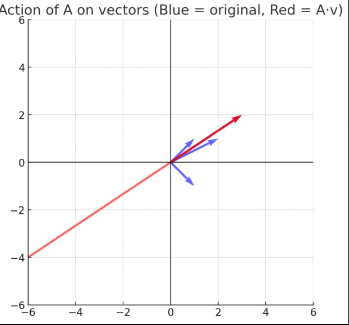
\includegraphics[height=0.5\textheight, keepaspectratio]{fig5.7.9.png}
    \label{figure_1}
\end{figure}
 
\end{document}